%==============================================================================
%  ENGR 2405 - Electrical Circuits I
%  Lab 7
%
%  Compile with pdfLaTeX (or XeLaTeX / LuaLaTeX).
%  If you use the listings code blocks, no extra setup is needed.
%==============================================================================
\documentclass[11pt]{article}

%------------------------- Packages -------------------------------------------
\usepackage[utf8]{inputenc}
\usepackage[T1]{fontenc}
\usepackage[margin=1in]{geometry}     % page margins
\usepackage{amsmath,amssymb}          % math
\usepackage{graphicx}                 % \includegraphics for schematics/scope shots
\usepackage{float}                    % [H] figure placement
\usepackage{booktabs}                 % nicer tables
\usepackage{siunitx}                  % \SI{5}{\ohm}, \SI{10}{\milli\second}, etc.
\usepackage{listings}                 % SciLab / netlist code blocks
\usepackage{xcolor}
\usepackage{caption}
\usepackage[hidelinks]{hyperref}
\usepackage{titlesec}

%------------------------- Section styling ------------------------------------
\titleformat{\section}{\Large\bfseries}{}{0pt}{}
\titlespacing*{\section}{0pt}{1.4em}{0.6em}

%------------------------- Code listing style ---------------------------------
\definecolor{codebg}{RGB}{245,245,245}
\definecolor{codecomment}{RGB}{0,128,0}
\definecolor{codekw}{RGB}{0,0,180}
\lstset{
    backgroundcolor=\color{codebg},
    basicstyle=\ttfamily\small,
    breaklines=true,
    frame=single,
    framesep=4pt,
    keywordstyle=\color{codekw}\bfseries,
    commentstyle=\color{codecomment}\itshape,
    showstringspaces=false,
    captionpos=b,
    tabsize=2,
}
\definecolor{codestr}{RGB}{163,21,21}      % strings
\definecolor{codenum}{RGB}{120,120,120}    % numbers

% --- MATLAB (uses the listings built-in language) -------------------------
\lstdefinestyle{matlab}{
    language=Matlab,
    stringstyle=\color{codestr},
}

% --- SciLab (custom: listings has no built-in SciLab language) -------------
\lstdefinelanguage{Scilab}{
    morekeywords={
        function,endfunction,if,then,else,elseif,end,for,while,do,
        select,case,break,continue,return,clc,clear,disp,mprintf,
        printf,zeros,ones,eye,linspace,inv,det,sum,length,size,abs,
        sqrt,real,imag,exp,sin,cos,tan,plot,plot2d,xlabel,ylabel,
        title,legend,grid,poly,roots,find,pause,error,warning,log
    },
    sensitive=true,
    morecomment=[l]{//},          % line comment
    morecomment=[s]{/*}{*/},      % block comment
    morestring=[b]",              % double-quoted strings
    morestring=[b]',              % single-quoted strings
}
\lstdefinestyle{scilab}{
    language=Scilab,
    stringstyle=\color{codestr},
}

% --- LTSpice netlist (custom: SPICE directives & comments) -----------------
\lstdefinelanguage{LTspice}{
    morekeywords={
        .tran,.op,.dc,.ac,.step,.param,.model,.lib,.include,.inc,
        .meas,.measure,.save,.backanno,.end,.ends,.subckt,.global,
        .ic,.nodeset,.options,.option,.func,.temp,.four,.noise,.tf
    },
    sensitive=false,
    morecomment=[l]{*},           % lines beginning with * are comments
    morecomment=[l]{;},           % inline ; comments
    morestring=[b]",
}
\lstdefinestyle{netlist}{
    language=LTspice,
    keywordstyle=\color{codekw}\bfseries,
    basicstyle=\ttfamily\small,
}

%==============================================================================
\begin{document}

%------------------------- Title block ----------------------------------------
\begin{center}
    {\LARGE\bfseries Lab 7 -- Transient Response}\\[0.8em]
    {\large <Your Name>}\\[0.3em]
    {\large <Lab Date (date you did the lab)>}
\end{center}
\vspace{1em}

%------------------------------------------------------------------------------
\section*{Description}
% Enter a brief description of the lab. This can be taken from the lab
% assignment itself.

In this lab we study the transient response of a first-order RC circuit by using
it as the timing element of an op-amp relaxation oscillator. The RC time constant
sets the rate at which the capacitor voltage charges and discharges, and the
op-amp, operating as a comparator in saturation, flips its output each time the
capacitor voltage crosses the reference set by a resistive feedback divider. The
output is therefore a square wave whose period depends only on the RC time
constant and the divider ratio. We use this oscillator to alternately flash a red
and a green LED at a chosen frequency. In Task~1 we build the oscillator with
fixed resistors sized for a \SI{1}{\hertz} blink rate and measure the two input
node voltages on the scope. In Task~2 we replace the divider with a
\SI{10}{\kilo\ohm} potentiometer and tune the circuit to \SI{2}{\hertz}, first at
the original RC value and then with the feedback resistor halved.

%------------------------------------------------------------------------------
\section*{Procedure}
% Describe the in-lab procedure you followed. Summarize it or number the steps.

\begin{enumerate}
    \item Measured each resistor and capacitor with the bench DMM/LCR before
          building, to record actual component values and rule out a bad part as
          a later source of error.
    \item Built the relaxation oscillator from the prelab schematic on the
          breadboard: a \SI{741}{} op-amp powered from \SI{+5}{\volt} and
          \SI{-5}{\volt} rails, the feedback divider $R_1$ (\SI{7.5}{\kilo\ohm})
          and $R_2$ (\SI{2.4}{\kilo\ohm}) from the output to the non-inverting
          input, and the RC branch ($R = \SI{10}{\kilo\ohm}$, $C =
          \SI{100}{\micro\farad}$) from the output to the inverting input.
    \item Connected the red and green LEDs in anti-parallel across the output
          through a current-limiting resistor, so one LED conducts on the positive
          output swing and the other on the negative swing.
    \item Powered the circuit and confirmed the two LEDs alternated at roughly one
          blink per second.
    \item \textbf{Task 1.} Probed the non-inverting node $V_1(t)$ and the
          inverting node $V_2(t)$ with the oscilloscope and recorded, for each: the
          oscillation frequency and the peak-to-peak voltage. Captured both
          waveforms.
    \item \textbf{Task 2, Step 1.} Replaced $R_1$ and $R_2$ with the
          \SI{10}{\kilo\ohm} potentiometer wired as a divider, then adjusted the
          wiper until the circuit oscillated at \SI{2}{\hertz}. Captured the
          waveform, removed the pot, and measured the two resistances $R_1$ and
          $R_2$ that the wiper produced. Computed the corresponding
          $\gamma = R_2/(R_1+R_2)$.
    \item \textbf{Task 2, Step 2.} Replaced the RC feedback resistor $R$ with half
          its value (\SI{5}{\kilo\ohm}), reinserted the potentiometer, and
          re-adjusted the wiper for \SI{2}{\hertz}. Captured the waveform, removed
          and measured $R_1$ and $R_2$, and computed the new $\gamma$.
\end{enumerate}

%------------------------------------------------------------------------------
\section*{Calculations}
% Put in any calculations you made. If you used SciLab, paste your program and
% its runtime printout here. Include any reconciliation equations (e.g. mesh
% currents to branch currents) if they are not part of your SciLab output.

\textbf{Circuit operation.}
Because the RC feedback makes $V_1$ and $V_2$ depend on the output in different
ways, the two inputs are never equal and the op-amp runs in saturation, giving an
output $V_o = \pm V_{sat}$. The non-inverting input is set by the resistive
divider, with no current into the op-amp:
\[
    \frac{V_1-0}{R_2}+\frac{V_1-V_o}{R_1}=0
    \;\Rightarrow\;
    V_1 = V_o\,\frac{R_2}{R_1+R_2} = \gamma V_o,
    \qquad
    \gamma = \frac{R_2}{R_1+R_2}.
\]
The inverting input is set by the RC branch charging toward the output:
\[
    C\frac{dV_2}{dt}+\frac{V_2-V_o}{R}=0
    \;\Rightarrow\;
    \frac{dV_2}{dt}+\frac{V_2}{RC}=\frac{V_o}{RC}.
\]

\textbf{The two saturation cases.}
When $V_2<V_1$ the output holds at $V_o=+V_{sat}$ and $V_2$ charges toward
$+V_{sat}$:
\[
    V_2(t)=V_{sat}+\bigl(V_2(0)-V_{sat}\bigr)e^{-t/RC}.
\]
When $V_2>V_1$ the output holds at $V_o=-V_{sat}$ and $V_2$ decays toward
$-V_{sat}$:
\[
    V_2(t)=-V_{sat}+\bigl(V_2(0)+V_{sat}\bigr)e^{-t/RC}.
\]
Each time $V_2$ reaches the reference $V_1=\gamma V_o$ the comparator switches and
the other case takes over, so the circuit oscillates.

\textbf{Period and frequency.}
Taking one half cycle that starts at $V_2(0)=-\gamma V_{sat}$ with $V_o=+V_{sat}$,
the switch happens when $V_2(t)=+\gamma V_{sat}$:
\[
    \gamma V_{sat}=V_{sat}+\bigl(-\gamma V_{sat}-V_{sat}\bigr)e^{-t/RC}
    \;\Rightarrow\;
    e^{-t/RC}=\frac{1-\gamma}{1+\gamma}.
\]
Solving for the half-period and using $\tau=RC$:
\[
    t=-\tau\ln\!\left(\frac{1-\gamma}{1+\gamma}\right),
    \qquad
    T=2t,
    \qquad
    f=\frac{1}{T}.
\]
The frequency depends only on $\tau$ and $\gamma$, so choosing $R_1$ and $R_2$
sets the blink rate.

\textbf{Component selection.}
The design targets are $f\approx\SI{1}{\hertz}$ with $RC=\SI{1}{\second}$ and
$R_1+R_2\approx R=\SI{10}{\kilo\ohm}$. From $RC=\SI{1}{\second}$ with
$R=\SI{10}{\kilo\ohm}$,
\[
    C=\frac{1}{R}=\frac{1}{\SI{10}{\kilo\ohm}}=\SI{100}{\micro\farad}.
\]
Setting $f=\SI{1}{\hertz}$ (so $T=\SI{1}{\second}$, $t=\SI{0.5}{\second}$) with
$\tau=\SI{1}{\second}$ gives
\[
    \frac{1-\gamma}{1+\gamma}=e^{-0.5}=0.6065
    \;\Rightarrow\;
    \gamma=0.245.
\]
With $R_1+R_2=\SI{10}{\kilo\ohm}$ this is $R_2\approx\SI{2.45}{\kilo\ohm}$,
$R_1\approx\SI{7.55}{\kilo\ohm}$. The nearest standard values are
$R_1=\SI{7.5}{\kilo\ohm}$ and $R_2=\SI{2.4}{\kilo\ohm}$, which give
$\gamma=0.2424$ and a predicted $f\approx\SI{1.01}{\hertz}$.

\textbf{Expected node voltages.}
Using the ideal saturation level $V_{sat}=\SI{5}{\volt}$: $V_1$ is a square wave
that sits at $\pm\gamma V_{sat}=\pm\SI{1.21}{\volt}$, and $V_2$ ramps
exponentially between the same two limits. Both therefore have
$V_{pp}=2\gamma V_{sat}=\SI{2.42}{\volt}$.

% --- SciLab program ---
\begin{lstlisting}[style=scilab, caption={SciLab design check for the oscillator frequency}]
// Lab 7 - relaxation oscillator design check
R1 = 7.5e3;      // non-inverting divider, top
R2 = 2.4e3;      // non-inverting divider, bottom
R  = 10e3;       // RC feedback resistor
C  = 100e-6;     // RC feedback capacitor

gamma = R2 / (R1 + R2);
tau   = R * C;
thalf = -tau * log((1 - gamma) / (1 + gamma));   // one saturation case
T     = 2 * thalf;
f     = 1 / T;

mprintf("gamma = %.4f\n", gamma);
mprintf("tau   = %.4f s\n", tau);
mprintf("T     = %.4f s\n", T);
mprintf("f     = %.4f Hz\n", f);
\end{lstlisting}

% --- SciLab runtime printout ---
\begin{lstlisting}[caption={SciLab runtime output}]
 gamma = 0.2424
 tau   = 1.0000 s
 T     = 0.9892 s
 f     = 1.0109 Hz
\end{lstlisting}

\textbf{Task 2 targets.}
For \SI{2}{\hertz} ($t=\SI{0.25}{\second}$) at the original $\tau=\SI{1}{\second}$,
the required ratio is
\[
    \frac{1-\gamma}{1+\gamma}=e^{-0.25}=0.7788
    \;\Rightarrow\;
    \gamma\approx0.124.
\]
After halving $R$ to \SI{5}{\kilo\ohm} the time constant drops to
$\tau=\SI{0.5}{\second}$, so holding \SI{2}{\hertz} requires
\[
    \frac{1-\gamma}{1+\gamma}=e^{-0.5}=0.6065
    \;\Rightarrow\;
    \gamma\approx0.245.
\]
So halving the feedback resistor calls for a larger $\gamma$ (a larger $R_2$
fraction) to keep the same blink rate; these two values are the targets for the
measured potentiometer settings.

%------------------------------------------------------------------------------
\section*{Simulations}
% Paste (a screenshot is best) your LTSpice schematic and the netlist. Include
% simulation results (graphic outputs, etc.). Node voltages / branch currents
% may be shown on the schematic if the image stays uncluttered; otherwise paste
% the "Simulation Run Results" table here.

The oscillator was simulated in LTSpice using the \texttt{UniversalOpAmp2} part,
powered by two DC sources wired to ground with opposite polarity to create the
$+V_{cc}$ and $-V_{cc}$ rails at \SI{+5}{\volt} and \SI{-5}{\volt}. The directive
\texttt{.ic V(Vo)=1} seeds the output so the circuit starts switching, and a
transient run of three to five periods (a few seconds) shows the steady
oscillation of $V_o$, $V_1$, and $V_2$.

\begin{figure}[H]
    \centering
    \fbox{\parbox[c][4cm][c]{0.8\textwidth}{\centering\itshape \fbox{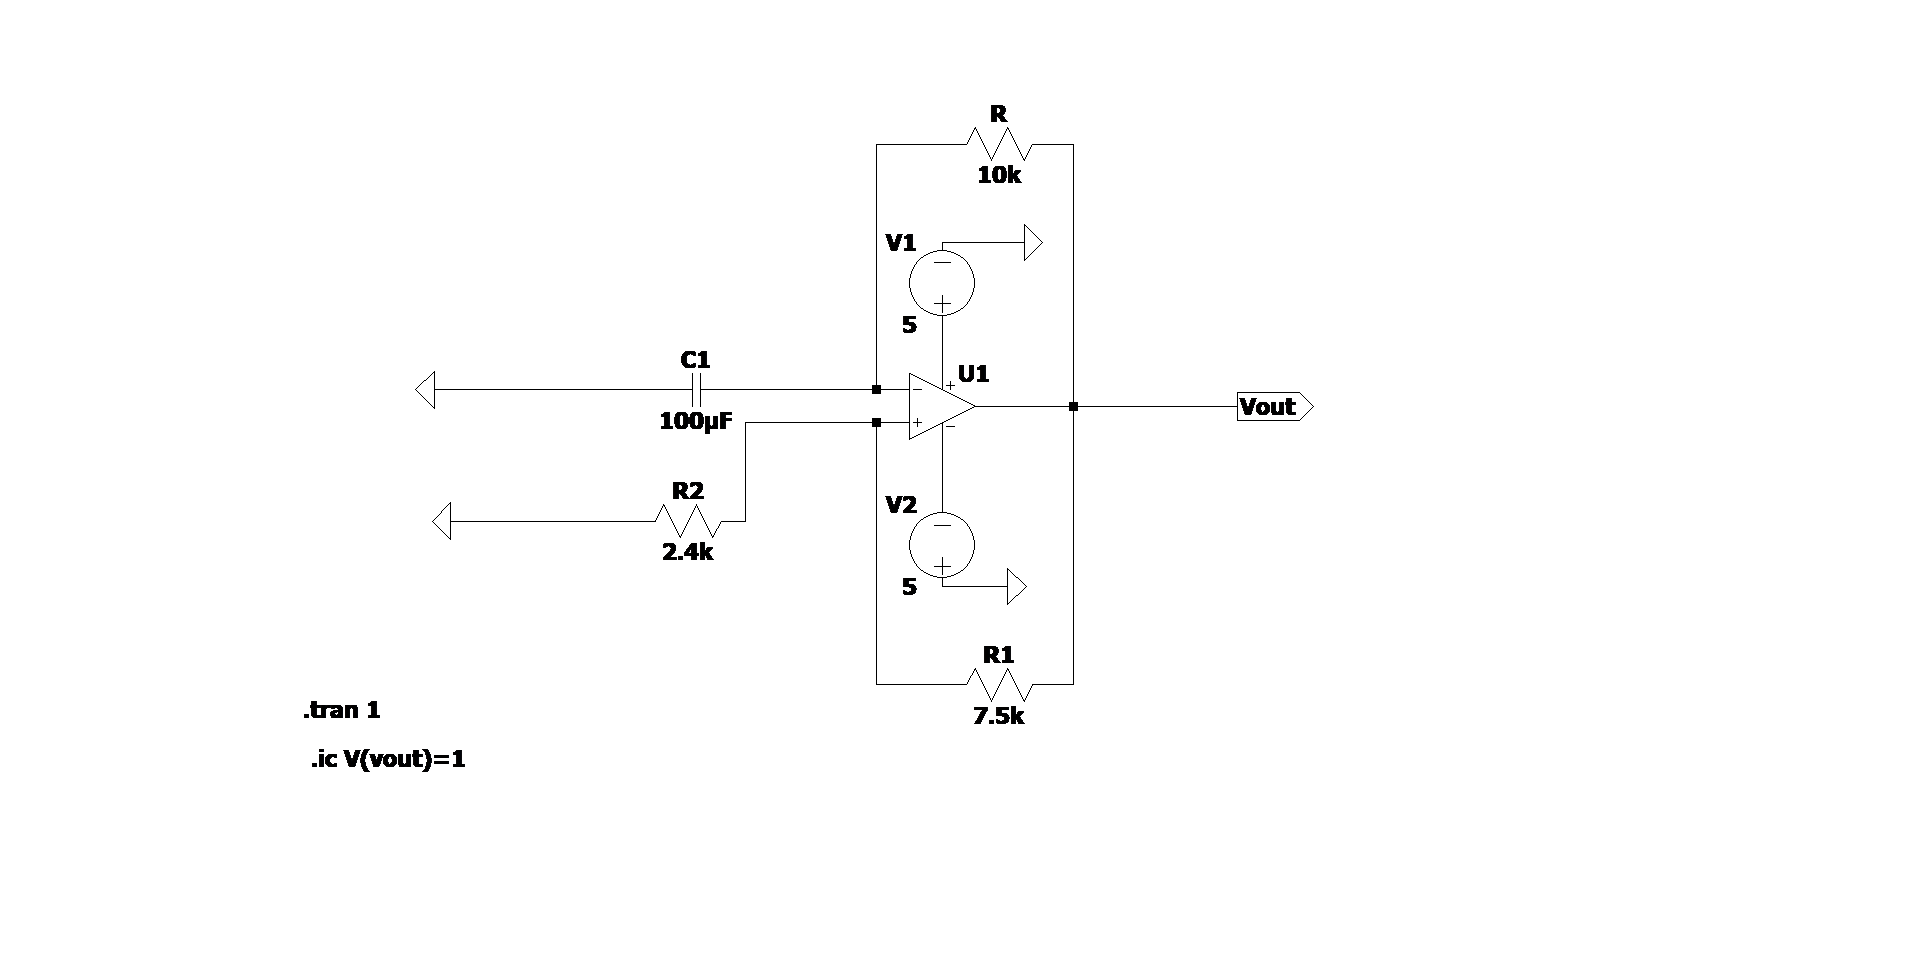
\includegraphics[width=0.8\textwidth]{lab07-circuit.png}}}}
    \caption{LTSpice schematic of the op-amp relaxation oscillator.}
    \label{fig:schematic}
\end{figure}

\begin{figure}[H]
    \centering
    % \fbox{\includegraphics[width=0.8\textwidth]{ltspice_waveform.png}}
    \fbox{\parbox[c][4cm][c]{0.8\textwidth}{\centering\itshape [Insert LTSpice waveform image here: $V_o$, $V_1$, $V_2$ vs.\ time]}}
    \caption{Simulated transient waveforms showing the output square wave $V_o$, the divider reference $V_1$, and the exponentially charging node $V_2$.}
    \label{fig:sim-waveform}
\end{figure}

\begin{lstlisting}[style=netlist, caption={LTSpice netlist (paste exported netlist here)}]
* G:\My Drive\lab07.asc
* Generated by LTspice 26.0.2 for Windows.
R1 Vout N003 7.5k
R Vout N001 10k
X§U1 N003 N001 N002 N004 Vout level2 Avol=1Meg GBW=10Meg Slew=10Meg Ilimit=25m Rail=0 Vos=0 En=0 Enk=0 In=0 Ink=0 Rin=500Meg ;§pnba In+)In-)V+)V-)OUT
C1 N001 0 100µF
R2 N003 0 2.4k
V1 N002 0 5
V2 0 N004 5
.tran 1
.ic V(vout)=1
* Library below included based on ModelFile attribute of instance X§U1 (C:\Users\Abdon Morales\AppData\Local\LTspice\lib\sym\OpAmps\UniversalOpAmp2.asy)
.lib UniversalOpAmp2.lib
.backanno
.end
\end{lstlisting}

%------------------------------------------------------------------------------
\section*{Measurements}
% Put in any measurements taken (Voltmeter, LCR, Oscilloscope, etc.) as a table
% of data or photos of oscilloscope images.

\textbf{Task 1.} Measured frequency and peak-to-peak voltage at the two input
nodes, compared against the prelab predictions. The oscilloscope read $V_1$ and
$V_2$ at essentially the same frequency (\SI{961.5}{\milli\hertz} and
\SI{961.1}{\milli\hertz}).

\begin{table}[H]
    \centering
    \caption{Task 1 -- measured node voltages vs.\ calculated ($V_{sat}=\SI{5}{\volt}$).}
    \begin{tabular}{lccc}
        \toprule
        Quantity & Calculated & Measured & \% Error \\
        \midrule
        Frequency          & \SI{1.01}{\hertz} & \SI{0.962}{\hertz} & $-4.9\%$ \\
        $V_1$ peak-to-peak & \SI{2.42}{\volt}  & \SI{2.14}{\volt}   & $-11.6\%$ \\
        $V_2$ peak-to-peak & \SI{2.42}{\volt}  & \SI{1.22}{\volt}   & $-49.6\%$ \\
        \bottomrule
    \end{tabular}
    \label{tab:task1}
\end{table}

\begin{figure}[H]
    \centering
    \fbox{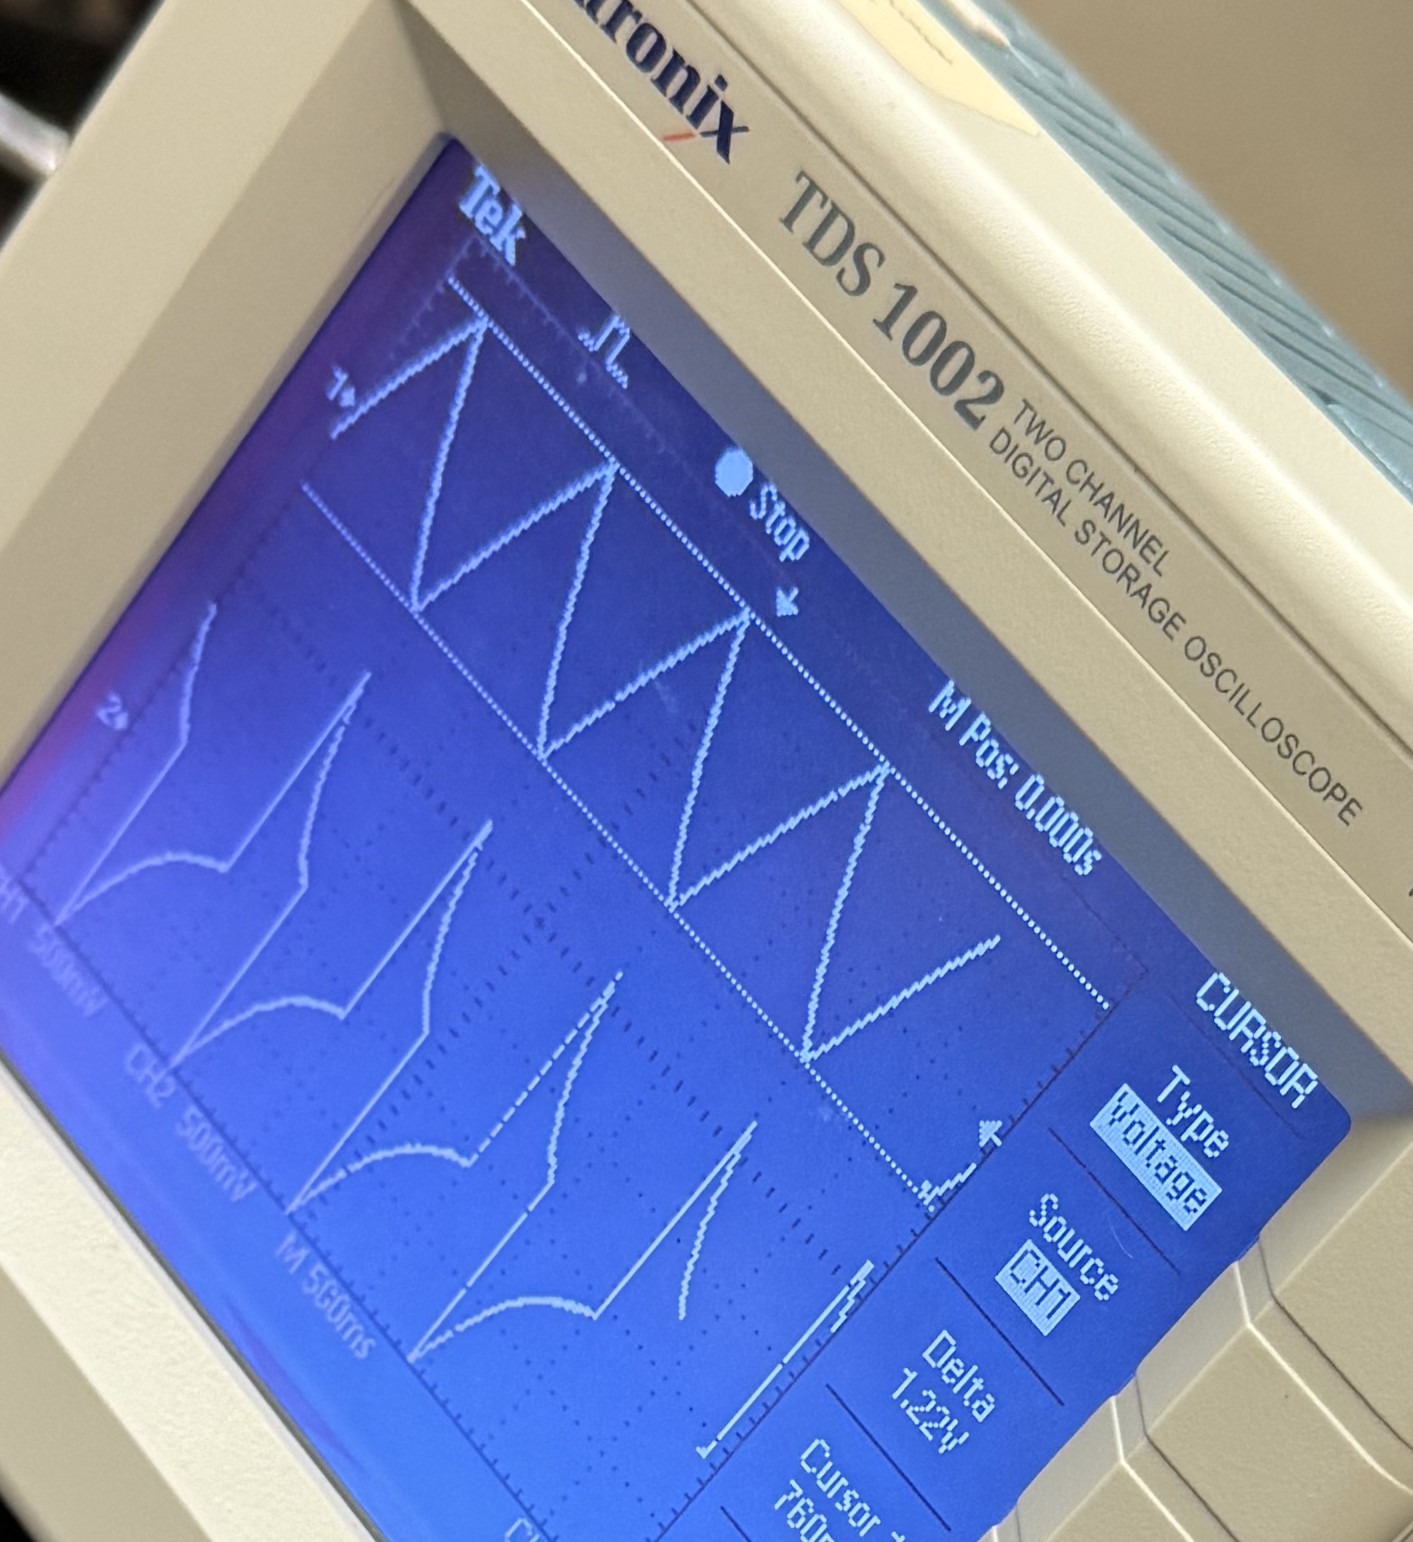
\includegraphics[width=0.72\textwidth]{fig_task1.jpg}}
    \caption{Task~1 measured waveforms at the \SI{1}{\hertz} configuration. CH1
    (triangle) is the capacitor node $V_2$ and CH2 is the non-inverting node
    $V_1$. The voltage cursors are set on $V_2$, reading its peak-to-peak at
    \SI{1.22}{\volt}. As in the Task~2 captures, the sloped CH2 tops are
    AC-coupling droop rather than a circuit effect.}
    \label{fig:scope-task1}
\end{figure}

\textbf{Task 2.} Potentiometer settings that produced \SI{2}{\hertz} oscillation,
with the resulting $\gamma$. Here $R_2$ is the ground-side segment of the pot (the
$V_1$-to-ground resistor) and $R_1$ is the feedback segment ($V_o$ to $V_1$), so
that $\gamma=R_2/(R_1+R_2)$ as defined in the prelab. For Step~2 the RC resistor
was set to a standard \SI{4.7}{\kilo\ohm} rather than an exact halving to
\SI{5}{\kilo\ohm}, so the \SI{2}{\hertz} target shifts from the prelab's
$\gamma\approx0.245$ to $\gamma\approx0.260$.

\begin{table}[H]
    \centering
    \caption{Task 2 -- potentiometer values at \SI{2}{\hertz}.}
    \begin{tabular}{lcccc}
        \toprule
        Configuration & $R_1$ & $R_2$ & $\gamma$ (measured) & $\gamma$ (target) \\
        \midrule
        Step 1: $R=\SI{10}{\kilo\ohm}$  & \SI{8.71}{\kilo\ohm} & \SI{1.34}{\kilo\ohm} & $0.133$ & $0.124$ \\
        Step 2: $R=\SI{4.7}{\kilo\ohm}$ & \SI{7.72}{\kilo\ohm} & \SI{2.49}{\kilo\ohm} & $0.244$ & $0.260$ \\
        \bottomrule
    \end{tabular}
    \label{tab:task2}
\end{table}

\begin{figure}[H]
    \centering
    \fbox{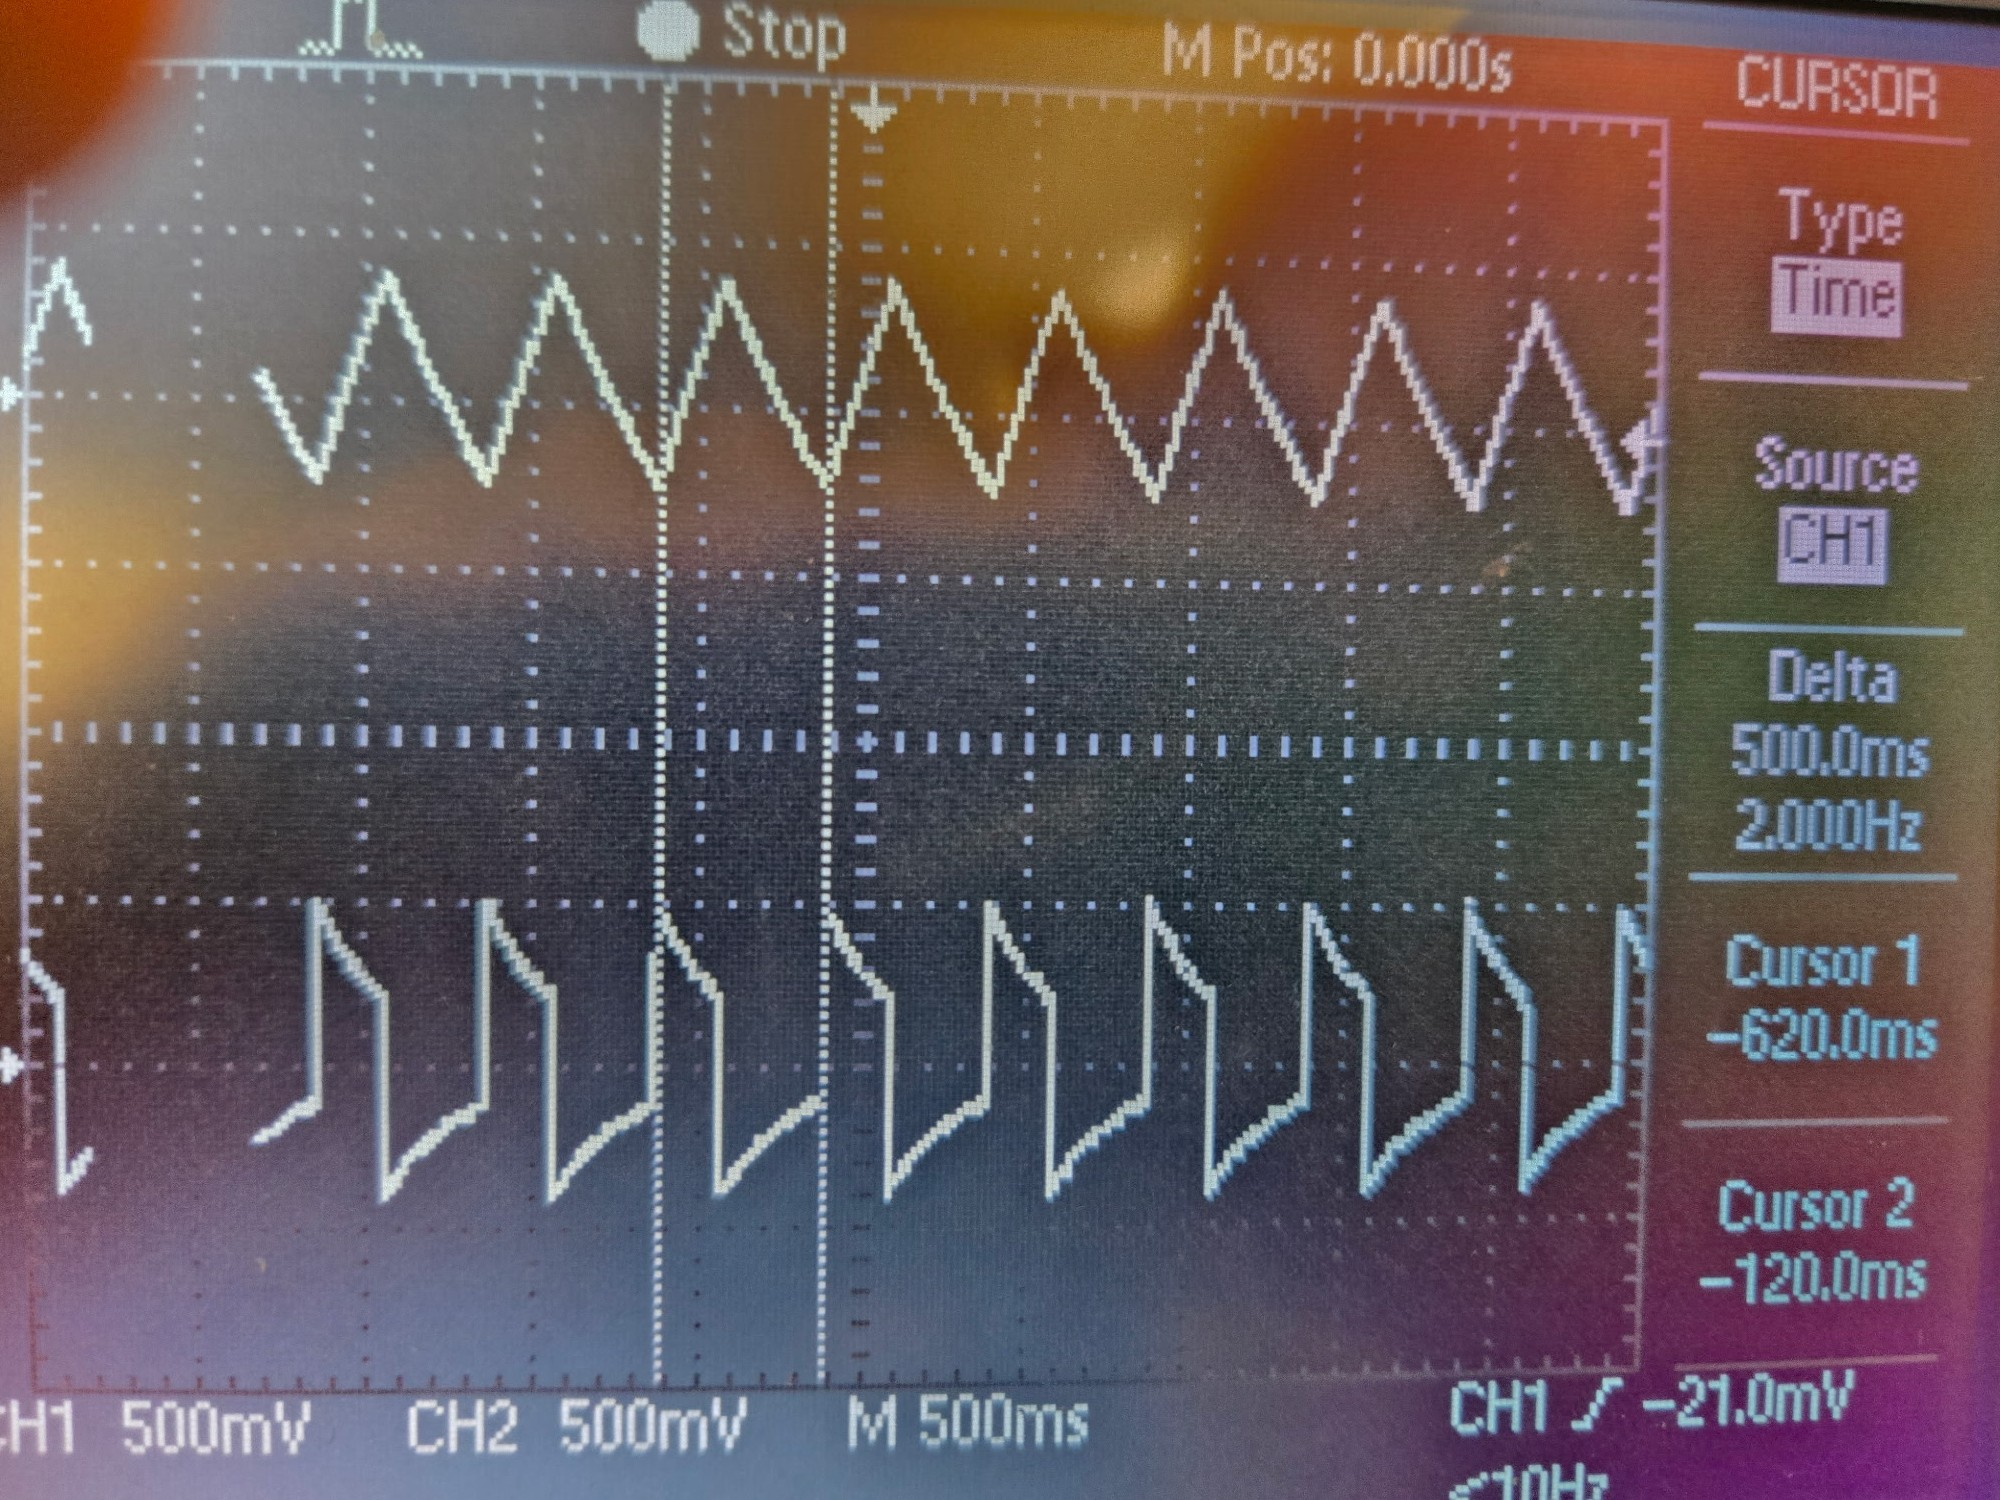
\includegraphics[width=0.85\textwidth]{fig_task2_step1.jpg}}
    \caption{Task~2 Step~1 at \SI{2}{\hertz} with the full \SI{10}{\kilo\ohm}
    feedback resistor. CH1 (triangle) is the capacitor node $V_2$; CH2 is the
    non-inverting node $V_1$. The sloped tops on CH2 are AC-coupling droop, not a
    circuit effect: the scope channels were AC-coupled (note the ``$<$\,10\,Hz''
    flag), whose high-pass corner near \SI{10}{\hertz} distorts the \SI{2}{\hertz}
    signal.}
    \label{fig:task2-step1}
\end{figure}

\begin{figure}[H]
    \centering
    \fbox{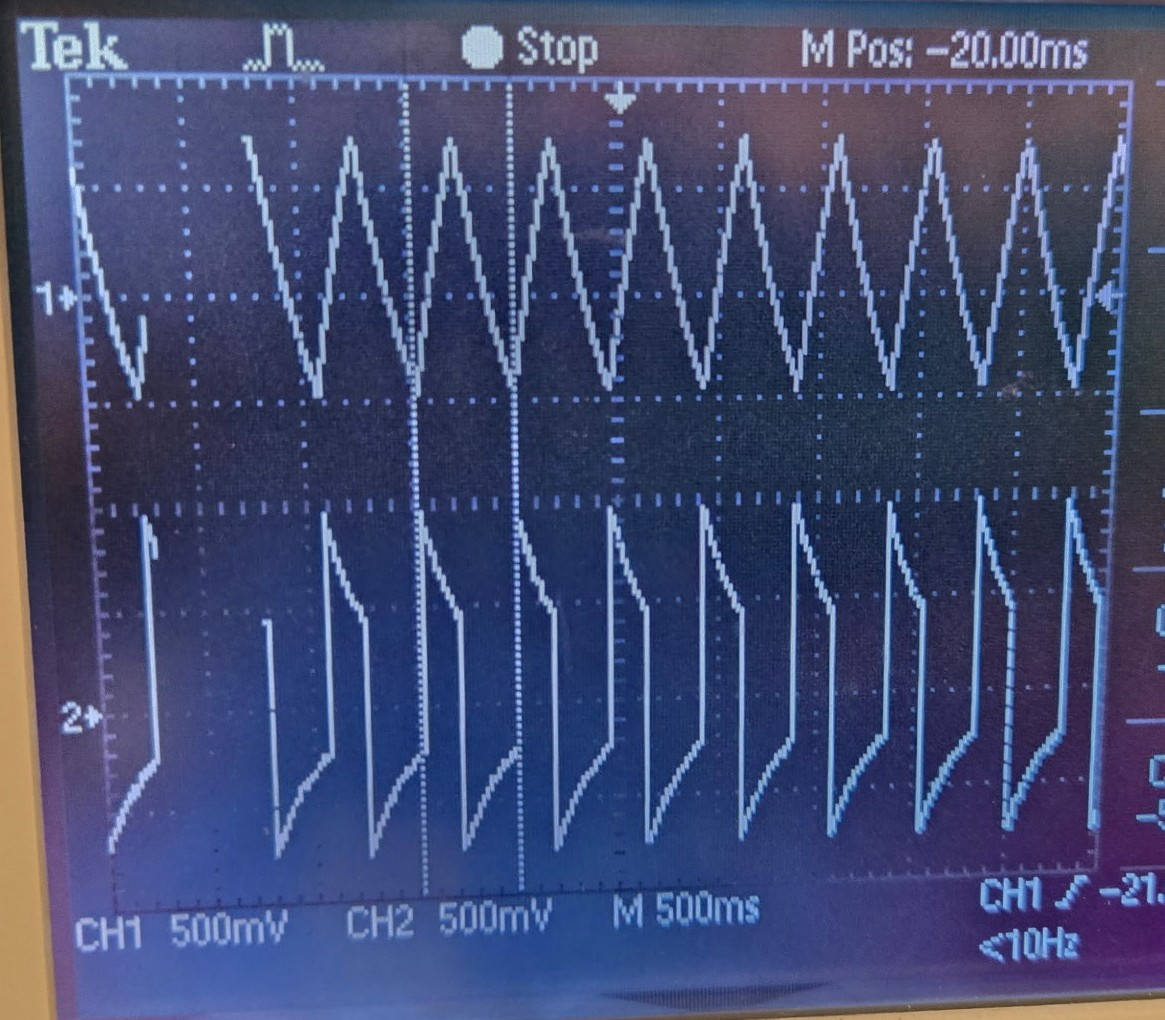
\includegraphics[width=0.85\textwidth]{fig_task2_step2.jpg}}
    \caption{Task~2 Step~2 at \SI{2}{\hertz} with the feedback resistor reduced to
    \SI{4.7}{\kilo\ohm}. Traces as in Figure~\ref{fig:task2-step1}; the CH2 droop
    is again AC-coupling distortion.}
    \label{fig:task2-step2}
\end{figure}

%------------------------------------------------------------------------------
\section*{Observations \& Discussion}
% List any anomalies or interesting observations. Discuss any discrepancies and
% their reasons. Answer any questions from the lab.

The circuit oscillated at \SI{0.962}{\hertz}, about \SI{4.9}{\percent} below the
predicted \SI{1.01}{\hertz}. Working backward from the measured period, the
effective divider ratio was $\gamma\approx0.254$ against the design value of
$0.242$, and the difference points to component tolerance: a slightly larger $R_2$
in the divider and a \SI{100}{\micro\farad} electrolytic running above its nominal
value both push $\tau=RC$ up and the frequency down. An electrolytic of this size
commonly carries a tolerance near $\pm\SI{20}{\percent}$, so a \SI{4.9}{\percent}
period shift is well within what the capacitor alone can account for.

The amplitudes tell a consistent story. The measured $V_1$ peak-to-peak was
\SI{2.14}{\volt}, about \SI{11.6}{\percent} below the \SI{2.42}{\volt} predicted
with an ideal $V_{sat}=\SI{5}{\volt}$. Since $V_1$ swings to $\pm\gamma V_{sat}$,
the measured value implies an actual saturation level of about \SI{4.4}{\volt},
meaning the \SI{741}{} output stops roughly \SI{0.6}{\volt} short of each rail
rather than reaching them. This is the expected behavior of a real \SI{741}{},
whose output cannot swing fully to the supply rails, and it is the main reason the
bench amplitudes sit below the simulated ones. The reduced swing also lowers the
switching thresholds slightly, which feeds back into the small frequency offset
noted above.

The one Task~1 result that at first did not fit this picture is the $V_2$
peak-to-peak, which came out at \SI{1.22}{\volt}, roughly half of $V_1$. Because
$V_2$ charges toward the output rail but reverses the moment it reaches the
switching threshold $\pm\gamma V_{sat}$, the same level $V_1$ sits at, its
peak-to-peak should be close to $V_1$'s \SI{2.14}{\volt} rather than half of it.
The captured waveforms explain the gap: the scope channels were AC-coupled, as
shown by the drooping tops on the square-wave trace and the ``$<$\,10\,Hz'' flag
the instrument displays. AC coupling applies a high-pass corner near
\SI{10}{\hertz}, which is well above the roughly \SI{1}{\hertz} fundamental of this
circuit, so it attenuates and distorts the low-frequency content of the signal.
That high-pass hits the smooth triangular $V_2$ harder than the sharp-edged $V_1$,
whose fast transitions still pass through and preserve its full edge-to-edge swing,
which is why $V_2$ reads low relative to $V_1$. Measured on DC coupling, $V_2$
would be expected to reach nearly the same peak-to-peak as $V_1$.

Task~2 returns to firmer ground and confirms the central prediction of the prelab.
With the full \SI{10}{\kilo\ohm} feedback resistor the pot settled at
$\gamma=0.133$ against a \SI{2}{\hertz} target of $0.124$, and after dropping the
RC resistor to \SI{4.7}{\kilo\ohm} it settled at $\gamma=0.244$ against a target of
$0.260$. Both land within about \SI{7}{\percent} of target, consistent with the
same resistor tolerance and capacitor offset seen in Task~1 together with the
resolution of setting the wiper by hand. More telling than the individual numbers
is the trend: lowering $R$ shortens $\tau$, which on its own would raise the
frequency, so holding \SI{2}{\hertz} forces $\gamma$ upward, and the measured
values climb from $0.133$ to $0.244$ exactly as the theory requires.

Taken together, the dominant source of error is the electrolytic capacitor
tolerance, which accounts for most of the frequency offset, followed by the
non-ideal \SI{741}{} saturation level, which explains the reduced amplitudes.
Resistor tolerance, the finite input bias current of the \SI{741}{} (so the
zero-input-current assumption is only approximate), and, for Task~2, the precision
of the potentiometer setting and the scope read-off all contribute at a smaller
level. The low $V_2$ peak-to-peak is a measurement artifact from AC input coupling
rather than a physical effect in the circuit, and the same coupling is visible as
the drooping square-wave tops in the Task~2 captures.

%==============================================================================
\end{document}
